\documentclass[11pt]{article}

\newcommand{\numpy}{{\tt numpy}}    % tt font for numpy
\usepackage[utf8]{inputenc}
\usepackage[english]{babel}
\usepackage{graphicx}
\topmargin -1.75in
\textheight 11in
\oddsidemargin -.75in
\evensidemargin -.75in
\textwidth 7in

\begin{document}

% ========== Edit your name here
\author{Anthony}
\title{VXB Vectors}
\maketitle

% ========== Begin answering questions here
\begin{figure}[h]
\centering
  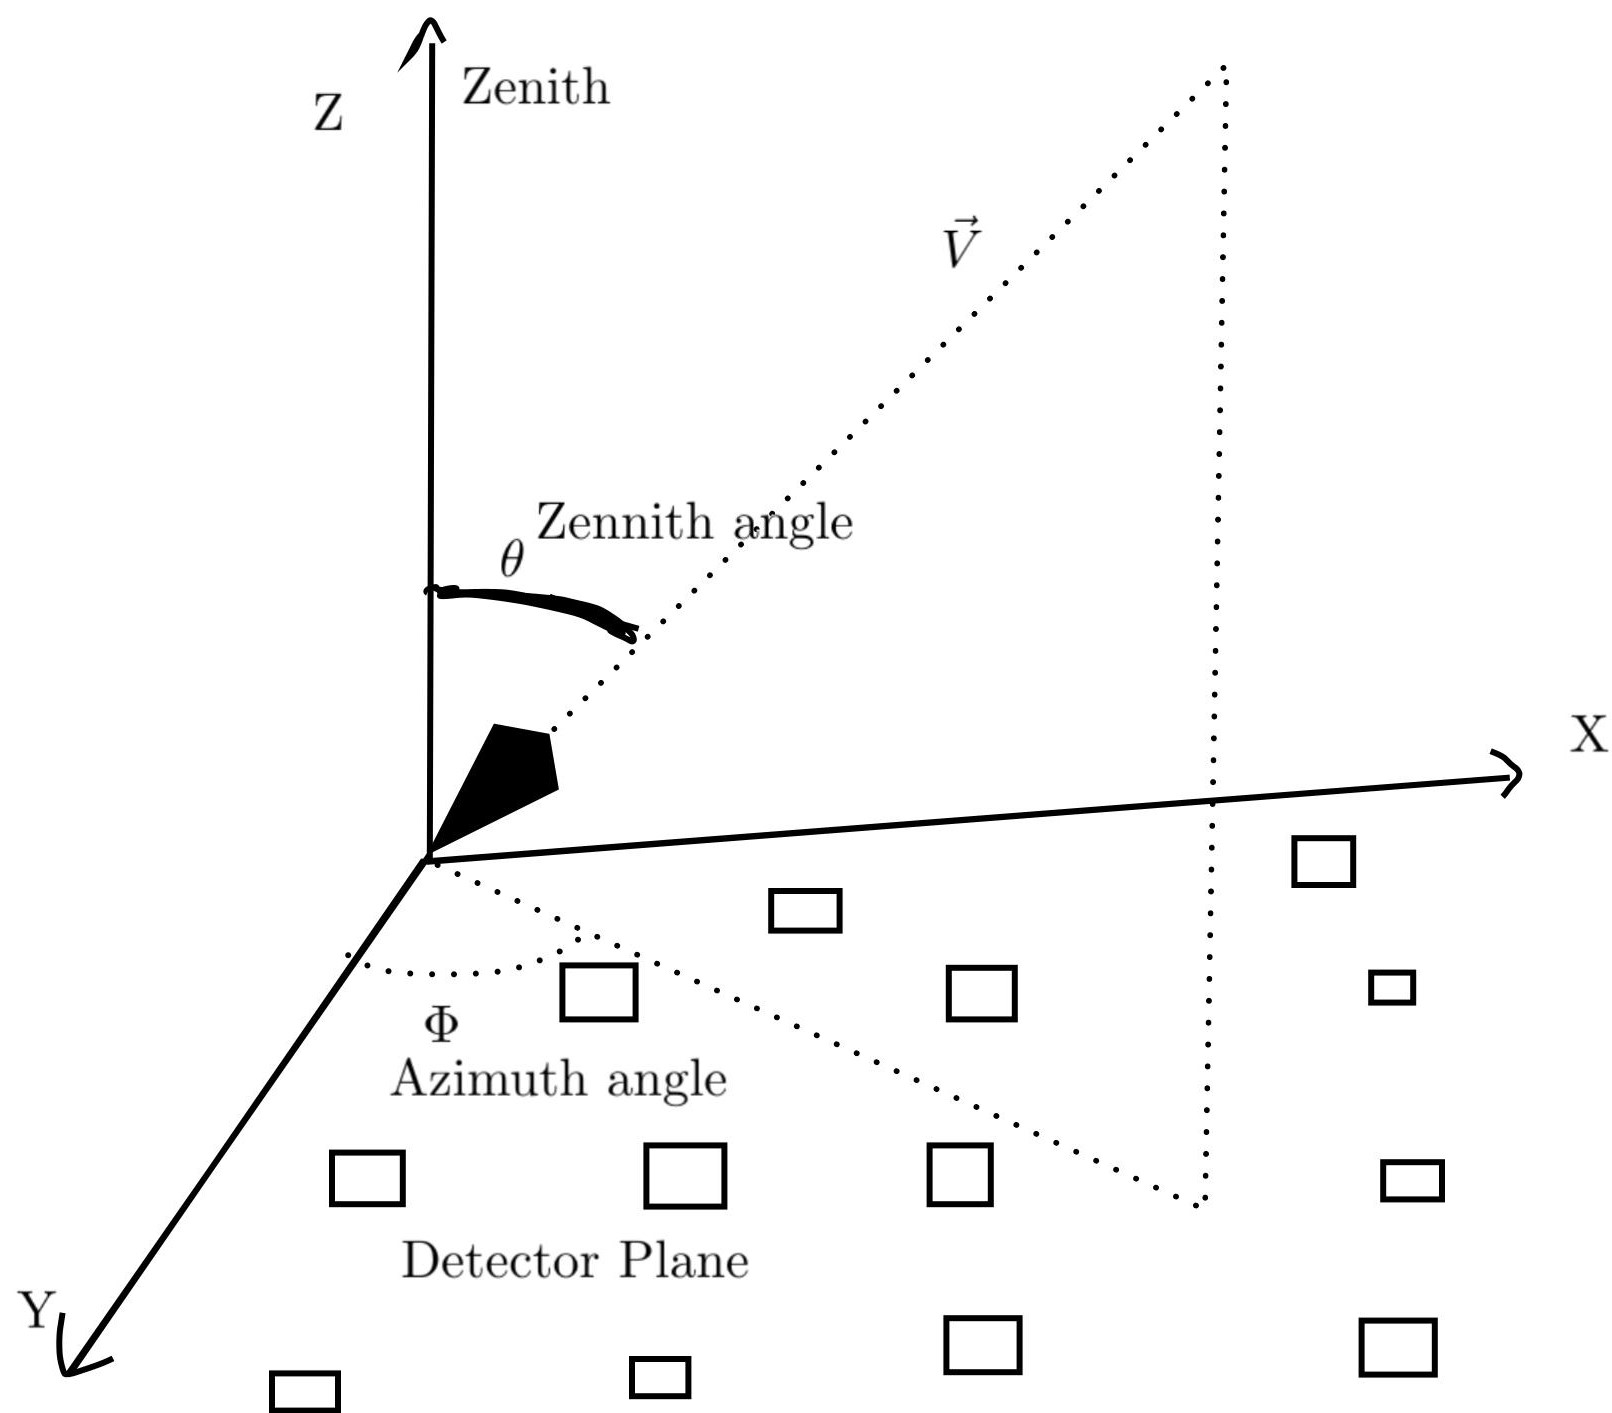
\includegraphics[scale=0.2]{vvv.JPG}
  \caption{Detector to shower plane }
  \label{fig:boat1}
\end{figure}

To start the coordinate transformation from the detector plane to the show plane, the unit vector of the incoming shower is to be needs to be described in the detector plane co-ordinates noting the zenith angle $\theta$  and the azimuth angle $\phi$. The shower $\mathbf{-\hat{V}}$ is then set to be the new zenith via the following transformation:
\begin{equation}
   \mathbf{-\hat{V}} = \frac{-1}{\left|V\right|}\left(
    \begin{array}{c}
    V\sin\theta \cos\phi \\ 	
    V\sin\theta \sin\phi \\ 
    V\cos\theta \\
\end{array} 
\right)
\end{equation}

To generate a second axis that is perpendicular to both the $\mathbf{\hat{B}}$ and and magnetic field  $\mathbf{\hat{B}}$, we get a cross product of both unit vectors.

\begin{equation}
    \mathbf{-\hat{V}}\times \mathbf{\hat{B}} = \left(
    \begin{array}{ccc}
    i & j & k \\ 	
   - \sin\theta \cos\phi & -\sin\theta \sin\phi  & -\cos\theta \\ 
    \frac{ B_x}{\left|B\right|}& \frac{ B_y}{\left|B\right|} &\frac{ B_z}{\left|B\right|}\\
\end{array} 
\right)
\end{equation}

The magnetic field unit $\mathbf{\hat{B}}$ vector can be written out more explicitly as:
\begin{equation}
   \mathbf{\hat{B}}=\frac{1}{\left|B\right|} \left(
    \begin{array}{c}
    B\sin\theta_B \\ 	
    0\\ 
    B\cos\theta_B \\
\end{array} 
\right),  \mbox{  where $\theta_B$ is the magnetic field inclination angle.}
\end{equation}

Considering negligible contribution in the y axis. The third axis is then a cross product of   $\mathbf{-\hat{V}}$ and $\mathbf{-\hat{V}}\times \mathbf{\hat{B}}$ to create a 3rd mutually perpendicular axis to both $\mathbf{-\hat{V}}$ and $\mathbf{-\hat{V}}\times \mathbf{\hat{B}}$ i.e. $\mathbf{-\hat{V}} \times\mathbf{-\hat{V}}\times \mathbf{\hat{B}}$. In an orientation that will give rise to the relationship $\mathbf{-\hat{V}} \times \left( \mathbf{-\hat{V}} \times\mathbf{-\hat{V}}\times \mathbf{\hat{B}}\right) = \mathbf{-\hat{V}}\times \mathbf{\hat{B}} $ , $\left(\mathbf{-\hat{V}}\times \mathbf{\hat{B}}\right) \times \left( \mathbf{-\hat{V}} \times\mathbf{-\hat{V}}\times \mathbf{\hat{B}}\right) = \mathbf{-\hat{V}}$ or check for orthogonality via the dot product that must equal 0.

% ========== Continue adding items as needed


\end{document}
\grid
\grid